\chapter{Referencial Teórico}

Este capítulo possui como propósito expor e definir tópicos pertinentes sobre o assunto abordado nesse trabalho, a fim de trazer maior contexto e entendimento sobre o unverso do assunto. Os conceitos que aqui serão abordados são: Conceitos Gerais (Aplicações \textit{Standalone} e Aplicações \textit{Web}), Componentes Gerais de uma aplicação \textit{Web} (\textit{Front-end}, \textit{Back-end} e Banco de Dados), padrão de projeto \textit{Model View Controller} (MVC), \textit{Ruby on Rails}, Escalabilidade e performance, e Cache com \textit{Ruby on Rails}.

Com a clarificação desses assuntos, será traga maior fundação teórica para que se siga com a pesquisa e com o caso de estudo, possibilitando assim maior embasamento durante as discussões referentes à problemática a ser estudada.

\section{Conceitos Gerais}

A seção Conceitos Gerais tem como objetivo introduzir conceitos fundamentais no escopo deste trabalho, a saber Aplicações \textit{Standalone} e Aplicações \textit{Web}. A apresentação destes dois tópicos permite com que sejam destacados aspectos pertinentes ao funcionamento de um \textit{software}, bem como a aplicação Brasil Participativo, através da comparação direta desses dois principais modelos de \textit{software} que operam no dia a dia, desde o computador pessoal de um estudante até os grandes \textit{mainframes} do mercado.

\subsection{Aplicações \textit{Desktop}}

Aplicações \textit{Desktop}, também chamadas de aplicações \textit{standalone} são softwares que atingem seu proposito de operacionalidade sem a necessidade de estarem conectados à internet, isto é, estas aplicações rodam em um computador ou dispositivo local que não necessariamente estão conectados à \textit{web}. Uma aplicação \textit{desktop} é autocontida, portanto, todo o código e os recursos utilizados por ela se encontram presentes no dispositivo que a executa.

Geralmente, aplicações \textit{desktop} são específicas à plataforma no qual foi projetada para operar, seja Windows, MacOS ou Linux. Dessa maneira, outro conceito pertinente que surge em meio às aplicações \textit{desktop} é a portabilidade. Portabilidade se refere à possibilidade de uma aplicação ser executada em diferentes ambientes com a mínima quantidade de ajustes que for necessária. Um \textit{software} dito portável pode executar, por exemplo, em Windows e MacOS com pouca ou nenhuma adaptação em seu código fonte, enquanto que, um software dito pouco portável, pode precisar ser reescrito do absoluto zero ou ter boa parte do seu código fonte adaptado para rodar em uma plataforma diferente da qual foi primariamente projetado \cite{tanenbaum1978guidelines}.

\subsection{Aplicações \textit{Web}}

Aplicações \textit{Web}, diferentemente de aplicações \textit{desktop}, são executadas no dispositivo do usuário através de outra aplicação, o \textit{Web Browser}. Aplicações \textit{Web} funcionam através do uso do modelo cliente/servidor, onde um dispositivo remoto, que possui os recursos da aplicação, os fornece para o dispositivo cliente, que serão exibidos para o usuário pelo \textit{browser}. Para que uma aplicação \textit{web} execute, é necessário que o dispositivo cliente esteja conectado à internet, ou, no mínimo à uma rede que tenha acesso ao dispositivo servidor. Geralmente, a conexão estabelecida no modelo cliente/servidor é através do protocolo \textit{Hypertext Transfer Protocol} (HTTP) ou sua variante \textit{Hypertext Transfer Protocol Secure} (HTTPS) \cite{conallen1999modeling}.

\subsubsection{Modelo Cliente/Servidor}

No modelo cliente/servidor, diferentemente de aplicações \textit{desktop} convencionais, o processamento de dados é feito no lado servidor. Portanto, na maioria das vezes, o lado cliente fica isento do processamento pesado de dados, sendo responsável apenas por exibir o resultado final ao usuário. Em geral, o fluxo seguido por uma aplicação cliente/servidor é iniciado pelo dispositivo cliente (usuário final), que solicita ao dispositivo servidor algum recurso; o servidor processa a requisição do cliente realizando o processamento necessário, e em seguida, devolve o recurso em um formato que o lado cliente consiga processar e exibir ao usuário final. Essa comunicação pode ocorrer através de diversos protocolos: \textit{File Transfer Protocol} (FTP) para transferência de arquivos, \textit{Simple Mail Transfer Protocol} (SMTP) para envio e recebimento de e-mails, e o já mencionado HTTP.

Cada protocolo dispõe de particularidades que derivam dos seus propósitos, fazendo com que cada um deles seja aplicável em um contexto específico. Entretanto, uma aplicação pode se beneficiar do uso de vários protocolos diferentes para cada uma de suas funcionalidades, isso a depender do propósito de cada um de seus módulos. Uma aplicação \textit{web} moderna, geralmente dispõe de funcionalidades para gerenciar recursos e exibi-los aos usuários utilizando o protocolo HTTP, em contrapartida, a própria entidade usuário pode ser considerada um recurso, onde, cada usuário tem um e-mail vinculado, permitindo que a aplicação envie informações utilizando o protocolo SMTP em algum outro momento oportuno.

A adoção do modelo cliente/servidor pode proporcionar à aplicação \textit{web} diversas características importantes, sendo a principal delas a centralização dos dados no lado servidor. Uma vez que os dados estejam centralizados no lado servidor, máquinas com mais recursos computacionais podem ser alocadas para que o processamento ocorra mais rapidamente e de forma desacoplada do ambiente do lado cliente, permitindo maior portabilidade da aplicação \cite{oluwatosin2014client}.

\section{Componentes Gerais de uma Aplicação \textit{Web}}

Uma aplicação \textit{web} moderna em geral pode ser vista dividida em duas partes: \textit{back-end} e \textit{front-end}. Ao contrário de aplicações \textit{standalone} convencionais que possuem a lógica de negócio altamente acoplada com a lógica de exibição, aplicações \textit{web} tendem a ter uma divisão mais clara nesse aspecto, permitindo com que a lógica de negócio não necessariamente interfira na renderização. Vale notar ainda a grande semelhança dessa abordagem com o modelo cliente/servidor \cite{gong2020architecture}. Outro importante componente no contexto de aplicações \textit{web} é o banco de dados, que cumpre o papel de persistir informações da aplicação. A seção Componentes Gerais de uma Aplicação \textit{Web} possui como objetivo introduzir cada um desses conceitos e elucidar seus papeis, trazendo maior clareza para cada um de seus papeis e como estes influenciam no funcionamento da aplicação \textit{web}, e consequentemente na sua performance.

\subsection{\textit{Front-end}}

O \textit{front-end} é a parte da aplicação \textit{web} responsável pela exibição dos dados e da interface de usuário. Idealmente, o \textit{front-end} lida apenas com a renderização de páginas, a lógica de \textit{design} da aplicação, sistema de rotas de páginas e recursos estáticos \cite{gong2020architecture}.

\subsection{\textit{Back-end}}

O \textit{back-end} é a parte da aplicação \textit{web} que lida com toda a lógica de negócio contida no escopo do \textit{software}. Todos os dados, bem como o processamento desses dados é realizado nessa camada. Do ponto de vista do funcionamento da aplicação como um todo, o \textit{back-end} possui como trabalho responder as requisições do usuário que vêm da camada do \textit{front-end}. Uma vez que o usuário pode enviar e requisitar dados, o \textit{back-end} deve ser capaz, através de um conjunto de métodos, processar a requisição e devolver uma resposta no menor tempo possível \cite{adam2019backend}.

A comunicação entre \textit{back-end} e \textit{front-end} pode ser realizada de diversas maneiras e com vários protocolos. Uma das formas mais adotadas como mecanismo de comunicação em aplicações \textit{web} modernas é a exposição de funções do \textit{back-end} por meio de \textit{Application Programming Interfaces} (APIs). As APIs podem ser vistas como interfaces de comunicação que visam abstrair a lógica de funcionamento por detrás de uma aplicação, expondo suas funcionalidades através de \textit{endpoints} que podem ser acessados por outras aplicações sem que a aplicação cliente precise saber como estas operam \cite{gough2021mastering}. 

\subsection{Banco de Dados}

Banco de Dados, nesse contexto, uma forma reduzida do termo Sistema Gerenciador de Banco de Dados, é uma classe de \textit{software} que lida com a manipulação e persistência de dados. Um banco de dados tem como objetivo fornecer aos seus usuários uma fonte de dados centralizada, com qualidade, integridade e segurança \cite{fry1976evolution}. Existem diversos tipos de bancos de dados, sendo revelantes para este trabalho: bancos de dados relacionais e bancos de dados de chave-valor.

\subsubsection{Banco de Dados Relacionais}

 mas o foco deste trabalho estará nos bancos de dados relacionais. Bancos de dados relacionais são bancos cujo os dados são guardados no formato de tabelas, também denominadas relações. As tabelas são compostas por colunas e linhas, semelhante a planilhas, onde cada linha representa um registro, denominado tupla, na tabela.

Bancos de dados relacionais permitem a criação de relacionamentos entre tabelas, sendo essa a motivação do termo "relacional". A maioria dos bancos de dados permitem manipular e consultar seus dados através do uso da linguagem de consulta \textit{Structured Query Language} (SQL) \cite{jatana2012survey}.

\subsubsection{Transações ACID}

No contexto de banco de dados, um importante conceito é o de transações. Uma transação é um agrupamento de operações realizadas pelo banco de dados, sendo a transação um conceito atômico, isto é, a menor instrução que o banco de dados realizará a mando do usuário. Existem características que um banco de dados pode ou não respeitar na sua implementação, estas são: atomicidade, consistência, isolamento e durabilidade (ACID). As propriedades ACID podem ser definidas da seguinte maneira:

\begin{itemize}
    \item Atomicidade: as operações envolvidas em uma única transação são executadas como uma só, implicando em que, caso uma falhe, a transação como um todo será dada como falha.
    \item Consistência: os dados presentes no banco de dados devem permanecer consistentes após a execução da transação.
    \item Isolamento: estados intermediários da transação não são visíveis por outras transações concorrentes, implicando que, uma transação não interferirá em outra.
    \item Durabilidade: quando uma transação é executada e chega ao fim, seus efeitos são persistentes. Caso ocorra interrupções ou falhas no banco de dados, uma transação completa não será afetada.
\end{itemize}

\cite{yu2009acid}.

\subsubsection{\textit{PostgreSQL}}

Segundo a documentação, o PostgreSQL é um gerenciador de banco de dados relacional \textit{open-source} que implementa e incrementa o padrão da linguagem SQL. O PostgreSQL implementa todos os princípios ACID desde 2001, além de oferecer \textit{plugins} que permitem o uso de outras funcionalidades não convencionais no contexto de banco de dados relacionais \cite{postgresql_about}.

\subsubsection{\textit{Redis}}

Bancos de dados chave-valor são sistemas gerenciadores de banco de dados que armazenam seus dados de forma não relacional utilizando de chaves e valores. Cada registro consistirá em uma chave e em um valor, podendo este ser armazenado tanto na memoria RAM, quanto no disco. Uma das principais características de bancos de dados chave-valor é a sua velocidade quando comparado com bancos relacionais. O \textit{Redis} é um banco de dados chave valor \textit{open-source} extremamente rápido que guarda seus dados em forma persistente no disco ou na memória RAM \cite{redis-in-action}.


\section{Padrão de Projeto \textit{Model-View-Controller}}

O MVC é um padrão de projeto que é considerado como um dos mais importantes na área da ciência da computação, pois este pode ser interpretado como algo mais próximo de uma filosofia de desenvolvimento de arquitetura de código, do que de um padrão de projeto que resolve instâncias de problemas de um domínio específico. O MVC possui uma grande abertura de interpretação e aplicação, podendo ser adotado desde subsistemas até aplicações inteiras. Essencialmente, o MVC é definido em três entidades: a \textit{model}, a \textit{view}, e a \textit{controller} \cite{Bucanek2009}.

As próximas subseções tem como objetivo descrever cada uma dessas entidades e qual papel desempenham dentro do contexto do padrão de projeto MVC.

\subsection{\textit{Model}}

A \textit{model} é a entidade do MVC que possui como preocupação encapsular informações do domínio do problema a ser resolvido pela aplicação. Um objeto de dados \textit{model} deve saber guardar, encapsular e abstrair os dados. Vale observar também que cada entidade idealmente não deve extrapolar suas funções, portanto, uma \textit{model} deve saber serializar seus dados, mas não deve saber como implementar uma funcionalidade de "salvar como" \cite{Bucanek2009}.

\subsection{\textit{View}}

Em poucas palavras, a \textit{view} é a entidade do MVC que apresenta informações na tela para o usuário final. Porém, a \textit{view} desempenha muitos outros papeis; na verdade, ela é a ponte entre o usuário e o sistema. Dessa forma, a \textit{view} é responsável por captar o \textit{input} do usuário e transformá-lo em comandos para o sistema processar. Outro aspecto importante é o escopo que uma \textit{view} pode atuar. No desenvolvimento de aplicações com o modelo MVC, objetos de \textit{view} podem ser generalistas ao ponto de saberem renderizar e lidar qualquer com qualquer tipo de texto, imagem ou mídia, ou podem ser específicos ao ponto de saberem renderizar apenas determinados objetos do sistema definidos no código pelo programador \cite{Bucanek2009}.

\subsection{\textit{Controller}}

A \textit{controller} é a entidade do MVC que implementa as ações do sistema. Como já mencionado, as \textit{models} sabem gerenciar seus dados a nível de persistência e abstração, as \textit{views} são responsáveis por coletar o \textit{input} do usuário para disparar as ações, estas que residem nas \textit{controllers}. Uma ação realizada por uma \textit{controller}, por exemplo, seria o comando "salvar como" de um dado armazenado dentro de uma \textit{model} \cite{Bucanek2009}.
Em geral, a comunicação realizada pelas entidades no modelo MVC pode ser visualizada na Figura \ref{fig:diagrama_mvc}.

\begin{figure}
    \centering
    \caption{Comunicação entre as entidades do MVC}
    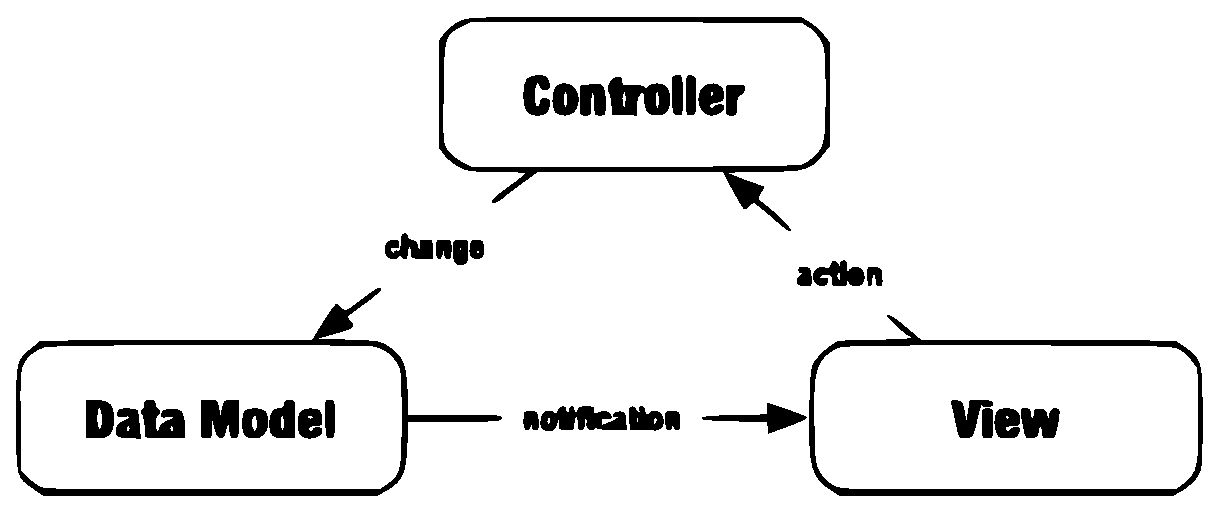
\includegraphics[width=\textwidth]{figuras/diagrama_mvc.eps}
    \fonte{\cite{Bucanek2009}}
    \label{fig:diagrama_mvc}
\end{figure}
\section{\textit{Ruby on Rails}}

O \textit{Ruby on Rails}, ou simplesmente \textit{Rails}, é um \textit{framework} de aplicação \textit{web} que fornece tudo o que é necessário para a criação de aplicações que seguem o modelo MVC e que utilizam de bancos de dados para armazenamento de suas estruturas e dados. O \textit{Rails} traz para cada uma das entidades do modelo MVC uma interface que provê as funcionalidades necessárias para que estas sejam implementadas em uma aplicação \textit{web}.

O \textit{Rails} traz duas interfaces para que o desenvolvedor consiga criar as \textit{models} no domínio de sua aplicação: o \textit{Active Record} e o \textit{Active Model}. Para as \textit{views}, o \textit{Rails} fornece a \textit{Action View}, que disponibiliza funcionalidades de geração de novas \textit{views} na aplicação. Para as \textit{controllers}, o \textit{Rails} fornece o \textit{Action Controller}. Cada uma dessas interfaces são exploradas em mais detalhes a seguir \cite{railsapi2023}.

\subsection{\textit{Active Record}}

O \textit{Active Record} é o "M" do modelo MVC no contexto do \textit{Rails}. De fato, o \textit{Active Record} é um padrão de projeto que precede o \textit{Rails}, este foi descrito por \textit{Martin Fowler} em seu livro \textit{Patterns of Enterprise Application}. No contexto de aplicações \textit{Rails}, o Active Record é caracterizado por sua responsabilidade de representar regras de negócio e dados, sendo uma ponte direta entre as \textit{models} da aplicação e o banco de dados, disponibilizando uma interface de \textit{Object Relational Mapping} (ORM) \cite{activerecord-basics}.

\subsubsection{\textit{Active Record como uma interface de ORM}}

O \textit{Active Record} provê, por padrão, uma interface de comunicação entre os objetos da aplicação com bancos de dados relacionais. Esta interface permite que o programador não necessite de escrever instruções SQL diretamente no código fonte da aplicação para buscar e persistir dados das \textit{models} no banco de dados \cite{activerecord-basics}. Além de prover esse mecanismo de interação com o banco, o \textit{Active Record} fornece diversas outras funcionalidades que permitem a configuração de validações sobre atributos da \textit{model}, além de prover mecanismos de \textit{callbacks} que são ativados automaticamente para os eventos básicos do ciclo de vida do objeto: criar, salvar, atualizar e destruir.

\subsection{\textit{Active Model}}

O \textit{Active Model} possibilita incorporar funcionalidades do \textit{Active Record} em uma classe \textit{Ruby} pura, sem a intenção de persistir seus atributos no banco de dados. O \textit{Rails} provê maneiras de se incluir separadamente cada uma dessas funcionalidades, permitindo com que a classe herde apenas os comportamentos desejados do \textit{Active Record} \cite{activemodel-basics}.

\subsection{\textit{Action View}}

As \textit{Action Views} no \textit{Rails} são usadas para renderizar o resultado de uma ação ou requisição processada pelo sistema. Em termos dos fundamentos de uma aplicação cliente/servidor, a função de uma \textit{Action View} é processar as informações a serem retornadas pelo sistema e compilá-las em um formato compreensível pelo usuário. O \textit{Rails} facilita essa renderização por meio de três componentes chave: \textit{templates}, \textit{partials} e \textit{layouts}.

\subsubsection{\textit{Templates}}

Os \textit{templates} atuam como um guia para a exibição das informações resultantes de uma ação. Por padrão, um \textit{template} da \textit{Action View} pode ser renderizado em diversos formatos, destacando-se entre eles: o \textit{HyperText Markup Language} (HTML), o \textit{JavaScript Object Notation} (JSON) e o \textit{Extensible Markup Language} (XML).

\subsubsection{\textit{Partials}}

As \textit{partials}, ou o termo mais completo \textit{template partials}, são exatamente o que o nome sugere: \textit{templates} parciais, ou seja, fragmentos de código que são extraídos para um arquivo separado e que podem ser reutilizados em diversas partes. O propósito das \textit{partials} é dividir o processo de renderização em partes para um melhor controle e permitir a reusabilidade, o que fomenta a filosofia do \textit{Don't Repeat Yourself} (DRY) \cite{actionview-overview}.

\subsection{\textit{Action Controller}}

O \textit{Action Controller} é uma parte essencial do padrão de arquitetura MVC, representando a letra "C". Ele gerencia as solicitações, processa dados provenientes da \textit{model} e gera a saída apropriada para exibição ao usuário. Em aplicações \textit{Rails} convencionais, o \textit{Action Controller} recebe a solicitação, interage com a \textit{model} para obter ou salvar dados, e utiliza a \textit{view} para criar uma saída em HTML ou qualquer outro formato necessário. Ou seja, o \textit{Action Controller} atua como intermediário entre os dados das \textit{models} e a apresentação ao usuário por meio das \textit{Action Views}. No \textit{Rails}, é possível definir \textit{actions} dentro das \textit{controllers} por meio de funções que recebem os dados da requisição e realizam as operações necessárias. Cada \textit{action} tem um \textit{template} de \textit{view} correspondente, fortalecendo a cooperação entre o \textit{Action Controller} e a \textit{Action View} \cite{actioncontroller-overview}.

\section{Performance e Escalabilidade}

A performance de uma aplicação \textit{web} pode ser avaliada de várias maneiras. Duas das maneiras mais conhecidas de aferir o nível de performance de uma aplicação é através do número de requisições processadas por segundo, também chamado de \textit{throughput} ou \textit{requests/second}, e o tempo gasto pela aplicação para responder a uma requisição. Uma boa aplicação visa manter seu \textit{throughput} alto e seu \textit{response time} baixo, de tal forma que a experiência do usuário seja positiva, a carga de uso seja suportada e a aplicação seja confiável em momentos de pico de acesso, evitando indisponibilidade. Sabe-se que 80\% do tempo gasto por uma aplicação no processamento de uma requisição é na execução operações no banco de dados, com consultas SQL, e na montagem da resposta para o usuário, com a renderização de \textit{templates} e criação do conteúdo compilado. \cite{jugo2014analysis}.

A aplicação de soluções web em diversas áreas de negócio, como vendas online, destaca o conceito de escalabilidade em contextos de software. Com o aumento da demanda e do acesso de usuários, é crucial que uma aplicação web possa expandir-se mediante a adição de recursos computacionais. Embora não haja um consenso claro sobre a definição de escalabilidade, geralmente é compreendida como a capacidade de uma aplicação aumentar seu \textit{throughput} por meio da incorporação eficiente de recursos de hardware. Essa capacidade é uma propriedade do sistema de software, fortemente influenciada pela arquitetura adotada. Se a arquitetura não permitir o aumento do \textit{throughput} em um determinado nível de demanda com a incorporação de mais recursos, ela é considerada não escalável. \cite{williams2004web}. 
\section{Cache com Ruby on Rails}

Em aplicações web, especialmente no contexto do \textit{Rails}, o conceito de \textit{cache} refere-se à prática de armazenar conteúdos gerados durante o processamento de requisições para posterior utilização em requisições subsequentes. O \textit{Ruby on Rails} fornece em sua API uma interface única e genérica que possibilita maneiras de integrar-se com sistemas terceiros que atuam como bases de dados para armazenamento de \textit{cache}. Isso oferece ao programador a flexibilidade de escolher estratégias de como um dado específico será armazenado, tornando também a tarefa de definir a expiração dos dados armazenados mais simples, algo que, quando feito manualmente, é bastante suscetível a erros. Na seção \ref{sec:tipos_de_cache_no_ruby_on_rails} é explorada as maneiras que o \textit{Rails} permite com que o programador utilize sua interface de \textit{cache}, e na seção \ref{sec:bases_de_dados_para_cache_no_ruby_on_rails} são explicadas as principais interfaces disponibilizadas pelo \textit{Rails} para comunicação com bases de dados para \textit{cache} \cite{caching-with-rails-overview}.

\subsection{Tipos de cache no Ruby on Rails}
\label{sec:tipos_de_cache_no_ruby_on_rails}

O \textit{Ruby on Rails} fornece maneiras de se utilizar \textit{cache} com funcionalidades embutidas, ou com \textit{gems} que se integram com o \textit{framework} sem muita dificuldade. A seguir são descritas cada uma dessas maneiras com suas particularidades, pontos positivos e negativos.

\subsubsection{Page Caching}

O \textit{page caching} é uma estratégia de \textit{cache} fornecida pela \textit{gem}  \textit{actionpack-page\_caching}, que consiste em salvar o conteúdo de uma requisição em um arquivo estático que será servido como resultado nas próximas requisições. Dessa maneira, uma vez salvo o resultado de uma requisição específica, quando realizada uma nova requisição ao mesmo \textit{endpoint}, o arquivo salvo será servido pelo servidor, de tal forma que a requisição sequer será processada pela aplicação \textit{Rails}. Essa abordagem apesar de simples, possui potencial para reduzir bastante o \textit{response time} da aplicação para os \textit{endpoints} que forem armazenados.

Porém, esta estratégia funciona apenas para requisições \textit{get} e \textit{head} com retorno de código 200. A utilização desse mecanismo de \textit{cache} também não é recomendada para páginas que requiram autenticação, pois a aplicação \textit{Rails} precisa decidir se o remetente da requisição está ou não autorizado a receber o conteúdo solicitado \cite{actionpack-page-caching}.

A \textit{gem actionpack-page\_caching} está disponível em seu repositório oficial no endereço \href{https://github.com/rails/actionpack-page_caching}{https://github.com/rails/actionpack-page\_caching}.

\subsubsection{Action Caching}

O \textit{action caching} é similar ao \textit{page caching} no sentido de que a resposta inteira será armazenada. Essa estratégia de \textit{cache} é fornecida pela \textit{gem actionpack-action\_caching}. Entretanto, nessa abordagem a requisição passa a ser recebida pela aplicação \textit{Rails}, ao ponto que os filtros são executados antes do \textit{cache} ser servido. Isto é, caso o \textit{endpoint} consultado requira autenticação para decidir se um determinado recurso será ou não servido, por exemplo, as verificações serão realizadas na \textit{controller}, para só então o conteúdo em \textit{cache} ser servido.

O \textit{action caching} permite que o programador especifique diretamente o tempo de vida de um armazenamento de \textit{cache} a nível de \textit{actions} dentro da \textit{controller}, além de permitir especificar condições para decidir se o resultado de uma \textit{action} será ou não servido por \textit{cache} \cite{actionpack-action-caching}.

\subsubsection{Fragment Caching}

Aumentando ainda mais o nível de granularidade do armazenamento de informação em \textit{cache}, o \textit{Rails} fornece um mecanismo chamado \textit{fragment caching}. Com o \textit{fragment caching} é possível armazenar fragmentos específicos do \textit{template} de uma \textit{view}, ao invés de armazena-la por inteira. Essa abordagem é especialmente utilizada em trechos da \textit{view} onde objetos de \textit{models} são renderizados.

Quando o \textit{Rails} se depara com um fragmento de \textit{view} que exibirá informações de um objeto de uma \textit{model}, e que há a instrução de armazenar o resultado em \textit{cache}, uma chave única será criada com base na junção do nome da \textit{view}, o nome da \textit{model} do objeto em questão, o \textit{id} e o atributo \textit{updated\_at} do objeto, que representam a chave primária e o momento em que o objeto foi atualizado pela última vez, respectivamente. Caso não exista um valor já armazenado em \textit{cache} para esta chave, o fragmento será renderizado pela aplicação e o resultado será armazenado na memória com associação direta à essa chave \cite{caching-with-rails-overview}.

\subsubsection{Russian Doll Caching}

Ao utilizar a estratégia de \textit{fragment caching}, nos cenários onde existem objetos cuja renderização acontece de forma aninhada com outros objetos em uma relação de \textit{has\_many/belongs\_to}, se um dos objetos aninhados for alterado, ainda assim o fragmento armazenado em \textit{cache} não expirará, pois o objeto mais externo não terá seu atributo \textit{update\_at} atualizado, conforme a Figura \ref{fig:russian_doll_template_example}. Para resolver esse problema, o \textit{Rails} oferece uma estratégia de armazenamento de \textit{cache} chamada \textit{Russian Doll Caching}. Essa estratégia consiste em adicionar no código da \textit{model} aninhada a opção \textit{touch: true} conforme ilustrado na Figura \ref{fig:russian_doll_touch_true}. Dessa maneira, sempre que um objeto aninhado for atualizado, o objeto mais externo também será marcado como atualizado \cite{caching-with-rails-overview}.

\begin{figure}
    \centering
    \caption{Exemplo de \textit{template} que renderiza objetos com \textit{caches} aninhados}
    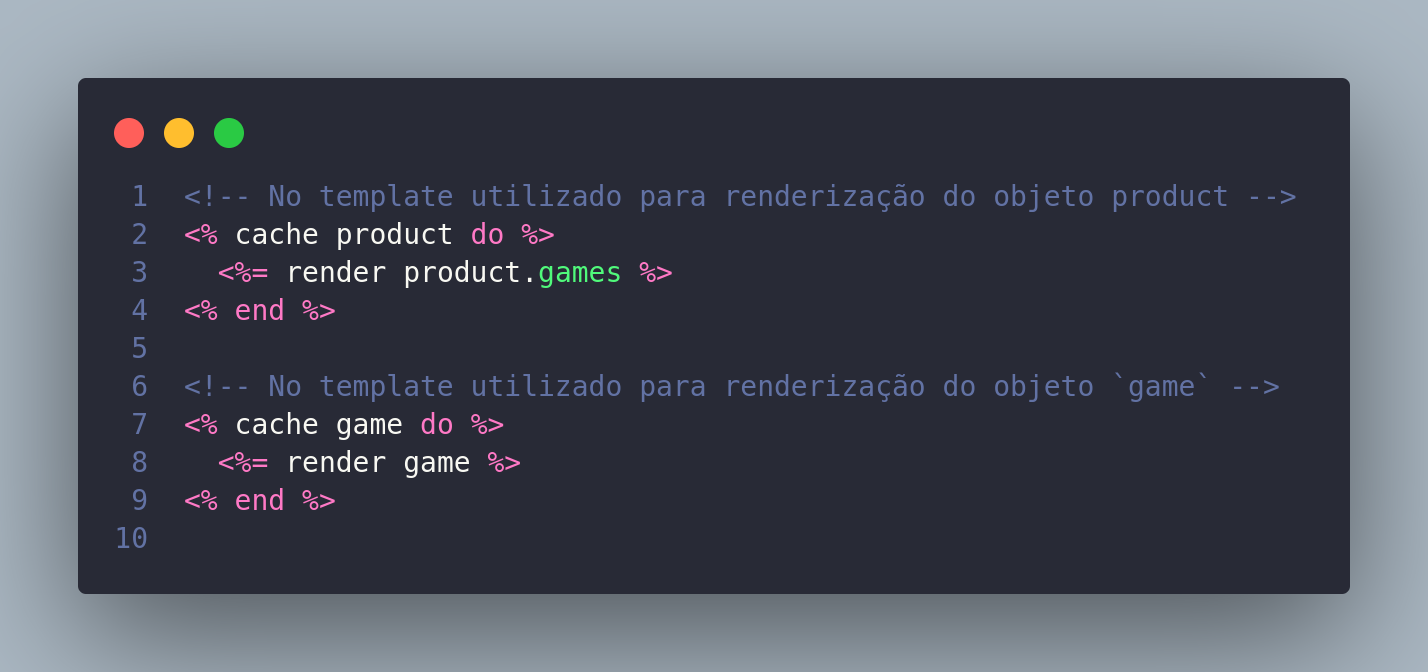
\includegraphics[width=0.7\textwidth]{figuras/russian_doll_template_example.png}
    \fonte{\cite{caching-with-rails-overview}}
    \label{fig:russian_doll_template_example}
\end{figure}


\begin{figure}
    \centering
    \caption{Inclusão da opção \textit{touch} na declaração de relacionamento entre \textit{models}}
    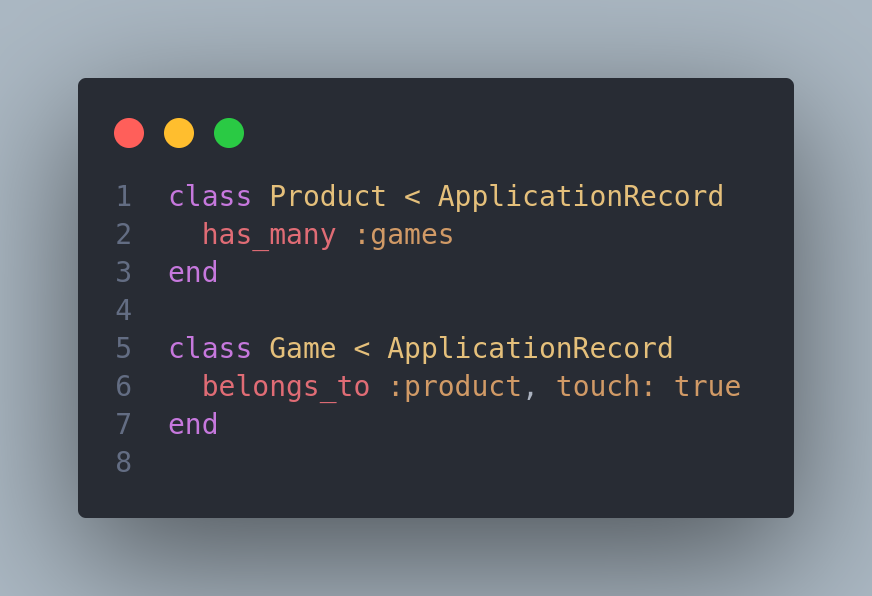
\includegraphics[width=0.7\textwidth]{figuras/russian_doll_touch_true.png}
    \fonte{\cite{caching-with-rails-overview}}
    \label{fig:russian_doll_touch_true}
\end{figure}

\subsection{Bases de dados para cache no Ruby on Rails}
\label{sec:bases_de_dados_para_cache_no_ruby_on_rails}

Como mencionado anteriormente, o \textit{Ruby on Rails} provê uma interface para comunicação com diversas tecnologias de armazenamento de \textit{cache}. Ele permite com que o programador especifique qual tecnologia deve ser utilizada na aplicação, e fornece uma interface que provê a fundação para interação com o sistema de \textit{cache}. Essa interface é o \textit{ActiveSupport::cache::Store}, que fornece métodos básicos para o programador: \textit{read}, \textit{write}, \textit{delete}, \textit{exist?}, e \textit{fetch}. Existem implementações dessa interface providas pelo \textit{Rails}, chamadas de \textit{Cache Store}, cujo propósito é operar com tecnologias de armazenamento conhecidas. Essas implementações são: o \textit{Memory Store}, o \textit{File Store}, o \textit{Mem \textit{cache} Store}, o \textit{Redis cache Store}, e o \textit{Null Store}; além de permitir o uso de \textit{Cache Stores} customizados.

\subsubsection{Memory Store}

O \textit{Memory Store} é uma tecnologia de armazenamento que utiliza a memória do próprio processo \textit{Ruby} em execução para guardar os registros. Esse \textit{cache store} possui as seguintes propriedades:

\begin{itemize}
    \item O tamanho do armazenamento é fixo, e deve ser especificado na configuração da aplicação;
    \item Sempre que faltar espaço para inserir novos registros, uma limpeza será realizada removendo os registros que não foram utilizados recentemente;
    \item No caso da aplicação estar rodando em múltiplos processos, um processo não terá acesso ao \textit{cache} do outro.
\end{itemize}

\subsubsection{File Store}

O \textit{File Store}, como o próprio nome sugere, utiliza o próprio sistema de arquivos para guardar os registros de \textit{cache}. Esse \textit{cache store} possui as seguintes propriedades:

\begin{itemize}
    \item O caminho do diretório utilizado para \textit{cache} é especificado na configuração da aplicação;
    \item No caso da aplicação estar rodando em múltiplos processos no mesmo \textit{host}, todos eles terão acesso ao mesmo \textit{cache}.
    \item O volume de dados utilizado pelo armazenamento de \textit{cache} cresce até que o disco se encontre cheio, sendo necessária a limpeza de registros antigos.
\end{itemize}

\subsubsection{Mem cache Store}

O \textit{Mem cache Store} é uma tecnologia de armazenamento de \textit{cache} baseada no \textit{memcached server} da \textit{Danga}. O \textit{Rails} utiliza a \textit{gem dalli} para operar com esse sistema de \textit{cache}, por padrão. Esse \textit{cache} \textit{store} possui a seguinte propriedade:

\begin{itemize}
    \item É possível utilizar um \textit{cluster} de servidores \textit{memcached}, porém, esses devem ser especificados na configuração da aplicação ou via variável de ambiente.
\end{itemize}

\subsubsection{Redis cache Store}

O \textit{Redis cache Store}, como o próprio nome sugere, é um \textit{cache store} que utiliza o \textit{Redis} como tecnologia de armazenamento de \textit{cache}. Esse \textit{cache store} possui as seguintes propriedades:

\begin{itemize}
    \item Dada a natureza do uso, é recomendado que se utilize um servidor \textit{Redis} dedicado para \textit{cache}.
    \item Servidores de \textit{cache Redis} permitem utilizar políticas de expiração de registros por: registro utilizado com menor frequência, ou registro que não é utilizado a mais tempo.
    \item O \textit{Redis cache Store} permite especificar parâmetros como: \textit{timeout} para conexão, \textit{timeout} para leitura, \textit{timeout} para escrita e tentativas de reconexão.
    \item O tempo gasto para criar ou reescrever um registro em \textit{cache} é pequeno, sendo as vezes mais vantajoso reescrever um registro do que esperar muito tempo para buscá-lo.
\end{itemize}
\section{Considerações Finais do Capítulo}

Este capítulo visou esclarecer conceitos relevantes sobre aplicações \textit{web} e seu funcionamento, a fim de permitir ser introduzida de maneira clara a abordagem de otimização de desempenho da plataforma Brasil Participativo. Essa plataforma foi desenvolvida em \textit{Ruby on Rails} e, atualmente, utiliza o PostgreSQL como recurso tecnológico para bancos de dados e o Redis para \textit{cache}.

Para compreender os desafios enfrentados pela plataforma e perceber a aplicabilidade das soluções propostas, é fundamental entender o funcionamento de aplicações cliente/servidor e o fluxo de operação de uma aplicação MVC, especialmente no contexto do \textit{framework} \textit{Ruby on Rails}. Como observado, grande parte do tempo consumido por uma aplicação web está relacionada à execução de operações no banco de dados e à compilação de dados para fornecer uma resposta ao cliente, etapas essas que podem ser otimizadas com a utilização de recursos de \textit{cache} fornecidos pelo próprio \textit{framework}.